\hltodo{A lot of material here. Need to sort it out}.

\hltodo{Split into two: BVS by calculating explicit Bayes factors, and when $p$ is large, need to use MCMC methods. Discussion on differences.}

Consider the linear regression model, where an $n \times 1$ response vector $\mathbf y = (y_1, \dots, y_n)$ relates to several predictors or covariates linearly through the following equation:
\begin{align}\label{eq:linmod1}
	\begin{gathered}
		\mathbf y = \boldsymbol\alpha + \mathbf X \boldsymbol\beta + \boldsymbol\epsilon \\
		\boldsymbol\epsilon \sim \text{N}(\mathbf 0, \psi^{-1}\mathbf I_n)
	\end{gathered}
\end{align}
where $\boldsymbol\alpha$ is the vector of intercepts ($\boldsymbol\alpha = \alpha\mathbf 1_n$, with $\mathbf 1_n$ being a vector of ones), $\mathbf X$ is an $n \times p$ matrix containing (column-wise) the $p$ observed explanatory variables, and $\boldsymbol\epsilon = (\epsilon_1, \dots, \epsilon_n)$ represents the errors. This linear model is undoubtedly familiar to any statistician, albeit written slightly differently. The constant term, or intercept, $\alpha$, is segregated from the vector of coefficients $\boldsymbol\beta$, thereby allowing us to discard the column of ones typically reserved for the intercept in the design matrix $\mathbf X$. Also, we have chosen to work with the precision of the errors $\psi$, instead of the usual variance $\sigma^2 = 1/\psi$. These errors are assumed to be identically distributed as normal with mean zero and variance $1/\psi$, although one could of course choose to abandon this assumption by specifying $\boldsymbol\Psi = (\psi_{ij})$ as the variance-covariance matrix instead. All of these are chosen as a matter of convenience, especially on notation, as we will see later on.

The ordinary least squares (OLS) estimates for the regression coefficients are given as $\hat{\boldsymbol\beta} = (\mathbf X^\top \mathbf X)^{-1} \mathbf X^\top \mathbf y$. This is obtained by maximising the normal likelihood of $\boldsymbol\beta$, but interestingly, the exact same solution is obtained by minimising the sum of squared errors - without having to set any distributional assumption on the errors. The form of the solution comes from only what is known to us: the data, $\mathbf X$ and $\mathbf y$.

The Bayesian approach to estimating the linear model takes a different outlook, in that it supplements what is already known from the data with additional information in the form of prior beliefs about the parameters, or simply, priors. Inference about the parameters are then performed on the posterior
\[
	f(\boldsymbol\Theta|\mathbf y) \propto {\color{gray}\overbrace{\color{black}f(\mathbf y|\boldsymbol\Theta)}^{\text{likelihood}}} \times {\color{gray}\overbrace{\color{black}f(\boldsymbol\Theta)}^{\text{prior}}}
\]
such as taking the mean, which is known as the Minimum Mean Squared Error estimate (MMSE), or the mode, which corresponds to the maximum a posteriori estimate (MAP). The Bayesian approach of MAP is similar to maximum likelihood, but differs only in the fact that the optimisation objective (the likelihood function) is augmented with a prior distribution about the parameters. It is critical then, that the prior chosen does not deter us in our cause of finding the correct estimates.

There are many ways of categorising different types of priors, but we like to think that priors can either be pure beliefs (subjective), or chosen according to some principle (objective). For instance, in estimating the chance of rain tomorrow, one might have their own personal feeling about this and elicit a certain probability based on no particular reason, but simply intuition. This is a subjective probability. However, one could also take into account historical data about the chances of rain on a particular day, somewhat more objectively. 

In any case, we would also like to categorise priors as either being informative or uninformative, although one could always question the actual informative value in eliciting subjective priors. As the name implies, informative priors aim to help nudge the parameter estimation in the right direction, assuming the prior itself is correct. On the other hand, uninformative priors provide little or vague information about the parameters, and in these cases, the data take over and the prior has little influence on the outcome. One example is the transformation invariant \citeauthor{Jeffreys1946}' \citeyearpar{Jeffreys1946} prior: $f(\theta) \propto  \sqrt{I(\sigma)}$, where $I(\sigma)$ is the Fisher information for $\sigma$. For a scale parameter\footnotemark $\ \sigma \in \mathbb{R}$, the \citeauthor{Jeffreys1946}' prior can be shown to be $f(\sigma) \propto 1/\sigma$, which isn't truly a distribution being a uniform distribution on the real line. Such distributions are known as improper priors. Regardless, these typically yield a proper posterior distribution which we can work with.

\footnotetext{A scale parameter $\sigma$ for a family of probability distributions satisfies $F(x; \boldsymbol\theta, \sigma) = F(x/\sigma; \boldsymbol\theta, 1)$, where $F$ is its cumulative distribution function.}

The type of prior that is of interest, at least for the purposes of Bayesian variable selection, is one which is objective and ideally informative. The I-prior fits this bill perfectly. A Gaussian I-prior on the regression coefficients $\boldsymbol\beta$ has some prior mean $\boldsymbol\beta_0$ and covariance matrix equal to the Fisher information for $\boldsymbol\beta$. This information theoretic prior for linear models has an intuitive appeal: when there is much Fisher information about the parameters, the covariance matrix for the prior will be large, and thus there will be little influence of the prior mean on the posterior estimate, and vice versa. We typically set the prior mean to be zero for this intuition to work favourably.

We realise there is an oddity in the classification of I-priors as informative. Previously, we alluded that a prior is said to be informative if it helps zone in on the ``correct'' estimate with the help of this prior, e.g. a normal prior assigned to a parameter with a small variance and prior mean close to the true value (assuming this is known somehow). Conversely, an uninformative prior would have a large variance. The I-prior is either informative or uninformative depending on the amount of Fisher information. Strictly speaking, since the informative-ness of the I-prior depends on the Fisher information, which in turn depends on the data, then technically the I-prior is considered to be uninformative as there really isn't any new information that the prior brings\footnote{This is a similar argument as to why the \citeauthor{Jeffreys1946}' prior is considered uninformative. \citet*{Liu2014} studied the Kullback-Leibler divergence between the prior and posterior, and noted that this divergence is maximised using \citeauthor{Jeffreys1946}' prior. In other words, this is the prior for which the data brings the maximal amount of information.}. Any mention of the informativeness of I-priors is then just semantic - in fact, the `I' in I-prior stands for information. 

Circling back to the topic of interest: variable selection, or more generally, model selection. In an ideal world, model selection entails searching the entire model space to find the ``best'' model based on minimising a certain criterion. There are many such criteria, making model selection a huge topic to cover fully. These include criteria such as (adjusted) $R^2$, Akaike's information criteria (AIC) and other similar information criteria, Mallow's $C_p$, ($k$-fold) cross-validation error, and many others. The obvious issue is that when the dimension of the full model is large, then a search of the entire model space may be computationally prohibitive or even downright unfeasible. 

The Bayesian philosophy to model evaluation may be thought of as follows: it is believed that a dataset $\mathbf Y$ had been generated from the pdf $f(\mathbf y|m_k, \boldsymbol\Theta_k)$, where $m_k$ is one of a set of $M=\{m_1, \dots, m_K\}$ models\footnote{We refer to these as models not in the usual sense - more precisely, each $m_k$ is a model class.}, and $\boldsymbol\Theta_k$ are the parameters associated with this model. The goal of model selection is then to infer which of the $K$ models had generated the data. The Bayesian approach allows us to assign priors to the parameters and the model index, i.e. $f(\boldsymbol\Theta_k|m_k)$ and $f(m_k)$ respectively, and thereby computing the posterior model distribution as
\begin{align*}
	f(m_k|\mathbf y)	&\propto f(\mathbf y|m_k)f(m_k) \\
						&\propto \int f(\mathbf y|m_k, \boldsymbol\Theta_k)
							f(\boldsymbol\Theta_k|m_k) \, \text{d}\boldsymbol\Theta_k \, f(m_k).
\end{align*}
The natural criteria for choosing $m_k$ is the one which gives the highest posterior probability. We refer to this model as the maximum probability model. 

If we are lucky, our problem may be simple enough that we are able to calculate all of the posterior probabilities, in which case the task is as simple as reading off the maximum probability model from a list of models with their corresponding probabilities. However, this is likely not the case, and we often have a large model set to consider. Even if the model set is small, we might find that the integral in the posterior is not analytically tractable. In either of these cases, Markov chain Monte Carlo (MCMC) methods is suitable to be used to overcome these issues of calculating the required posterior probabilities. In fact, MCMC methods can be quite efficient in the exploration of the model space because it  will favour models which have great potential of being the true model, and will tend to ignore those that have little to no potential. 

While the description we have just given for model selection is generic for most statistical models, variable selection is just a special case of model selection to where the model at hand is defined by the inclusion or exclusion of a finite number of variables. The linear regression model we were describing earlier is such an example. Much work has been done on Bayesian variable selection: \cite{George1993}, \cite{Kuo1998}, and \cite{Dellaportas2002} to name a few. We will be reviewing these methods later on, comparing similarities and differences, strengths and weaknesses, for it is these methods that we intend to improve on by using I-priors. The main motivation behind using I-priors in Bayesian variable selection is its suitability in accommodating to datasets with strong multicollinearity and being able to run with little to no prior information about the parameters.

In this section, we put our Bayesian thinking caps on. Earlier, we introduced the concept of Bayesian model evaluation. Variable selection is just a special case of this whereby a model is defined by the inclusion or exclusion of variables. The linear model \eqref{eq:linmod1} defined at the beginning is an example of this, and for the remainder of this paper, we will only consider models of this type. 

A model is defined as a subset of variables selected from the full set of variables $\{X_1, \dots, X_p \}$ and is linearly related to the response variables through the model equation in \eqref{eq:linmod1}. As each of the $p$ variables can either be selected or not selected, the size of the model space is $2^p$. Even for moderate $p$ we can see how the size of the model space can become exponentially large, such that a search of the entire space would be impractical. Note that we do not consider the intercept to be selectable. If this were the case, this would imply a model as having intercept equal to zero as being possible. For most practical modelling purposes, the intercept is almost always non-zero.

It would be useful to be able to index each of these $2^p$ possible models somehow. We do this by introducing the model identifier vector
\[
	\boldsymbol\gamma = (\gamma_1, \dots, \gamma_p).
\]
This vector of length $p$ contains elements which indicate whether or not that particular variable was selected. In other words, $\gamma_j = 1$ if $X_j$ was selected in the model, and $\gamma_j = 0$ otherwise for $j=1,\dots,p$. The full model, where all the variables are included in the model, is denoted by $\boldsymbol\gamma = (1, \dots, 1)$. The intercept only model is denoted by $\boldsymbol\gamma = (0, \dots, 0)$.

With this in mind, we can then assign priors to the model $f(\boldsymbol\gamma)$, and also to the parameters of the model $f(\boldsymbol\Theta|\boldsymbol\gamma)$. Ultimately, we are interested in two things:
\begin{enumerate}
	\item \textbf{Posterior inclusion probabilities} $\Prob[\gamma_j=1|\mathbf y]$ for variable $X_j$, for $j=1,\dots,p$. This gives us an indication of how often each variable was selected in the posterior models.
	\item \textbf{Posterior model probabilities} $\Prob[\boldsymbol \gamma=\boldsymbol \gamma_k|\mathbf y]$. This gives us a sense of how likely a particular model would appear a posteriori.
\end{enumerate}
The posterior inclusion probabilities can be thought of as the marginals of the posterior model probabilities across each variable. Also, as the distribution on the model probabilities are on a finite set, the posterior distribution is that of a probability distribution function, hence we speak of probabilities instead of densities.

These two types of quantities can be obtained by deriving the posterior distributions for the variable selection model if they are simple enough to be obtained. Sometimes, the relevant expressions are not available in closed form. Alternatively, MCMC methods such as Gibbs sampling can be employed to provide estimates of the quantities of interest. This is perhaps the preferred option, especially when $p$ is large such that the computation all of the $2^p$ posterior model probabilities takes an unfeasible amount of time. MCMC usually does not list out all of the $2^p$ probabilities, but instead just the ones which are substantial enough to be deemed important. Models not visited in the MCMC posterior state space are assigned probability zero. Monte-Carlo errors are inevitably introduced into the estimates, but a large enough MCMC run can control these errors.

\subsection{Overview of Bayesian variable selection methods}

We start with an overview of the available methods, in chronological order of appearance in the literature. There are many good in-depth reviews to these methods and the reader may find \cite{OHara2009} or \cite{Chipman2008} useful. 

\subsubsection{\texorpdfstring{\citeauthor{George1993}'s}{George and McCulloch's} Stochastic Search Variable Selection (SSVS)}

\begin{align}
	\begin{gathered} 
	y_i = \alpha + \beta_1 x_{i1} + \dots + \beta_p x_{ip} + \epsilon_i \\
	\epsilon_i \sim \text{N}(0, \psi^{-1}) \text{ iid} \\
	i = 1,\dots,n \\
	\\
	\text{\underline{Prior for $\boldsymbol\beta$}} \\
	\beta_j|\gamma_j \sim \gamma_j\text{N}(0,c^2_jt^2_j) + (1-\gamma_j)\text{N}(0,t^2_j) \\
	j=1,\dots,p
	\end{gathered}
\end{align}

One of the early works on Bayesian variable selection for linear models come from the \citeyear{George1993} paper by \citeauthor{George1993}. In it, they augmented the indicator variables $\boldsymbol\gamma$ into the prior for $\boldsymbol\beta$, while the linear model itself remained the same. The prior for $\beta_j$ is essentially one of two normal distributions, depending on whether or not variable $X_j$ was selected. 

The idea behind this type of prior is this: when variable $X_j$ is not important, then $\gamma_j$ should be equal to zero and the coefficient associated with it $\beta_j$ should be small and close to zero as possible. Therefore, the prior on $\beta_j$ should be normal with mean zero and have a small variance $t_j^2$. Conversely, when the variable $X_j$ is important, then $\gamma_j$ is one and $\beta_j$ should be non-zero, and thus the prior on $\beta_j$ should have a large variance $c_j^2 t_j^2$. In essence, $t_j$ and $c_j$ are tuning parameters that the user must choose. The authors give some suggested values for these tuning parameters: $\big(\text{SE}(\hat\beta_j)/t_j, c_j\big)$ = $(1,5)$, $(1,10)$, $(10,100)$, or $(10,500)$, where $\text{SE}(\hat\beta_j) = \sqrt{\hat\psi^{-1}(\mathbf X^\top\mathbf X)_{jj}}$ under the full model.

The priors on $\beta_j$ need not be independent of each other. Perhaps a more convenient notation for this prior is 
\[
	\boldsymbol\beta|\boldsymbol\gamma \sim \text{N}(\mathbf 0, \mathbf R_{\boldsymbol\gamma}\mathbf D \mathbf R_{\boldsymbol\gamma}), 
\]
where $\mathbf D = \mathbf I_p$, $\mathbf R_{\boldsymbol\gamma}=\text{diag}[a_jt_j]$ and $a_j = \gamma_j c_j + (1-\gamma_j)$, for $j=1,\dots,p$. The matrix $\mathbf D$ determines the independence of the $\beta_j$s. Setting this to be the identity matrix implies independence. On the other hand, \cite{George1993} proposed setting this proportional to the inverse sample correlation matrix in order to capture the design correlation.

\vspace{-0.5mm}
\subsubsection{\texorpdfstring{\citeauthor{Kuo1998}'s}{Kuo and Mallick's} sampler (KM)}

\vspace{-1mm}
\begin{align}
	\begin{gathered} 
		y_i = \alpha + \gamma_1\beta_1 x_{i1} + \dots + \gamma_p\beta_p x_{ip} + \epsilon_i \\
		\epsilon_i \sim \text{N}(0, \psi^{-1}) \text{ iid} \\
		i = 1,\dots,n \\
		\vspace{-0.5mm}\\
		\text{\underline{Prior for $\boldsymbol\beta$}} \\
		\beta_j \sim \text{N}(b_j,d_j^2) \\
		j=1,\dots,p
	\end{gathered}
\end{align}

Several years later in \citeyear{Kuo1998}, \citeauthor{Kuo1998} published their Bayesian variable selection model, commonly referred to as the independent sampler, so-called because of the independence of the $\beta_j$s and the $\gamma_j$s. Instead of having the $\gamma_j$s augmented into the prior, these are augmented into the model equation itself. Each term $\beta_j x_{ij}$ has its corresponding $\gamma_j$ multiplied to it. Therefore, when $\gamma_j=0$, the corresponding term drops out from the model.

The only hyperparameters one needs to choose for this model are the prior means and variances for the normal distributions of the $\beta_j$s, similar to the Bayesian approach for estimating linear models. These choices reflect one's prior beliefs about the coefficients. In the absence of prior information, one can simply set $b_j=0$, and choose $d_j=d$ such that $1/2 \leq d \leq 4$ after standardising the $\mathbf X$ variables. Otherwise, the user must choose an appropriate value of $d_j$ for each $j$ that would reflect the uncertainty of the estimate $\beta_j$ being zero.

The appeal of this method is its simplicity, and that also benefits the Gibbs sampling procedure, as the Gibbs conditional densities are easily worked out, and available in a recognisable closed form.

\subsubsection{\texorpdfstring{\citeauthor{Dellaportas2002}'s}{Dellaportas et al.'s} Gibbs Variable Selection (GVS)}
\label{sec:dellaportas}

\begin{align}
	\begin{gathered} 
		y_i = \alpha + \gamma_1\beta_1 x_{i1} + \dots + \gamma_p\beta_p x_{ip} + \epsilon_i \\
		\epsilon_i \sim \text{N}(0, \psi^{-1}) \text{ iid} \\
		i = 1,\dots,n \\
		\\
		\text{\underline{Prior for $\boldsymbol\beta$}} \\
		\beta_j|\gamma_j \sim \gamma_j\text{N}(b_j,d_j^2) + (1-\gamma_j)\text{N}(u_j,s^2_j) \\
		j=1,\dots,p
	\end{gathered}
\end{align}

The authors \cite{Dellaportas2002} worked on an improvement to the current Bayesian variable selection methods, a method which they call the Gibbs Variable Selection (GVS). \cite{Ntzoufras2008} provides an excellent reading about this method in his book, which also provides a good tutorial on using WinBUGS to estimate such models.

At first glance, their model looks like a cross between SSVS and KM, in that the $\boldsymbol\gamma$ indicators appear both in the model and in the prior. There are two priors for $\boldsymbol\beta$: one is the actual prior, and one which they call the ``pseudo prior''. This pseudo prior does not make its way into the posterior, and therefore does not influence the estimate at all. Instead, it is there just to make sampling more efficient, according to the authors. Why? When $\gamma_j$ is one, then $\beta_j$ is sampled from the posterior with the actual prior. This, coupled with the appropriate hyperparameters $b_j$ and $d_j$, should encourage $\beta_j$ to be non-zero. On the off-chance that $\gamma_j$ is zero when the variable $X_j$ is important, then $\beta_j$ is sampled from the posterior with a pseudo prior which is designed such that good values for $\beta_j$ are proposed. If the data (likelihood) also encourages $\beta_j$ to be non-zero, then there is a high chance that $\gamma_j$ will flip back to being one. In short, the pseudo prior helps flip the gamma in the right direction, if and when it needs to be flipped, and therefore spends less time being in the wrong state space. 

With this model you do need to choose several tuning parameters. As before, we can choose $b_j = 0$ and $d_j=d$ with large $d$ (after standardising $\mathbf X$) if no prior information. As for the pseudo prior hyperparameter, \cite{Dellaportas2002} suggests the following choices:
\begin{enumerate}
	\vspace{-3mm}
	\item $u_j=\hat\beta_j$, the estimates of a full pilot MCMC run, and correspondingly $s^2_j = \widehat{\text{Var}}(\hat\beta_j)$.
	\item $u_j=0$ and $s^2_j \propto d_j^2$, but kept low.
	\vspace{1mm}
\end{enumerate}

\begin{remark}
	In the long run, we expect the KM and GVS methods to give identical results if the same prior $N(b_j, d_j^2)$ for the $\beta_j$s are used. As mentioned, the pseudo prior in the GVS method merely improves efficiency of the Gibbs sampler.
\end{remark}

\subsubsection{Choices of priors}
\label{sec:priorchoices}

The main difference between the the three methods above, apart from the model structure itself, is the prior specified for $\boldsymbol\beta$, but the priors for the rest of the common parameters are and can be similar. The priors for the intercept $\alpha$ and precision $\psi$ are chosen as the conjugate normal-gamma prior, and the prior for each $\gamma_1, \dots, \gamma_p \in \{0,1\}$ is of course chosen to be Bernoulli:
\begin{align*}
	\begin{gathered}
		\text{\underline{Priors for $\boldsymbol{\gamma}$, $\alpha$, and $\psi$}} \\
		\gamma_j \sim \text{Bern}(p_j), \ j=1,\dots,p \\
		\alpha \sim \N(a,b^2) \\
		\psi \sim \Gamma(c,d)
	\end{gathered}
\end{align*}

Typically, in the absence of any prior knowledge, the hyperparameters are set to reflect an uninformative prior. For the normal-gamma, this implies the normal having mean $a=0$ and large variance $b^2$, while the gamma having both shape and scale parameters $c$ and $d$ small. Note that a $\Gamma(c,d)$ distribution becomes the Jeffrey's prior as $c$ and $d$ approaches zero. On the other hand one may actually have some prior knowledge about these and may set these hyperparameters accordingly. In any case, we are not too concerned about estimating the intercept and precision parameters. 

\stepcounter{todocounter}
\todo[caption={\thetodocounter. Investigate if letting the model estimate the common prior probability for the gamma variables will improve results.}]{Estimate common $p$}
For the Bernoulli prior on the indicator variables, we can appeal to the principle of indifference and set all $p_j = 1/2$, as each variable may either be selected or not selected. Another possibility is to let the model estimate this common probability $p_1=\cdots=p_p=p$ by assigning a hyperprior such as a beta distribution. The beta hyperprior can be chosen to be uninformative, such as Beta(1,1) (Uniform distribution) or Beta(1/2,1/2) (Jeffrey's prior). The user may also choose to code more complex relationship between the variables - e.g. if variable $X_1$ is included, then $X_2$ must be included - useful when performing variable selection on interaction effects. This way, the priors on $\gamma_1, \dots,\gamma_p$ will not be independent, and care must be taken when deriving the posteriors.

\subsection{The I-prior Bayesian variable selection model (I-prior)}

When we compare the three models side-by-side, there are obvious differences in the structure of the models. Things such as the structure of the parameter space, the amount of tuning parameters that need to be set, and how the two sets of parameters of interest $\boldsymbol\gamma$ and $\boldsymbol\beta$ behave in each model. Figure \ref{fig:modcompare} summarises these differences. 

However, in practice there isn't generally much to distinguish between these three models. It is more than likely that each of these methods will be optimal for a specific problem that the user faces, rather than one having an all-out advantage over the other in all situations. Having said that, these three methods have one thing in common, which is that they do not perform very well when faced with selection scenarios with correlated variables. This may be because of the use of independent $\boldsymbol\beta$ priors which lessens the posterior correlations, and thus smaller models tend to be selected \citep{George1993}.

\begin{figure}[ht]
	\centering
	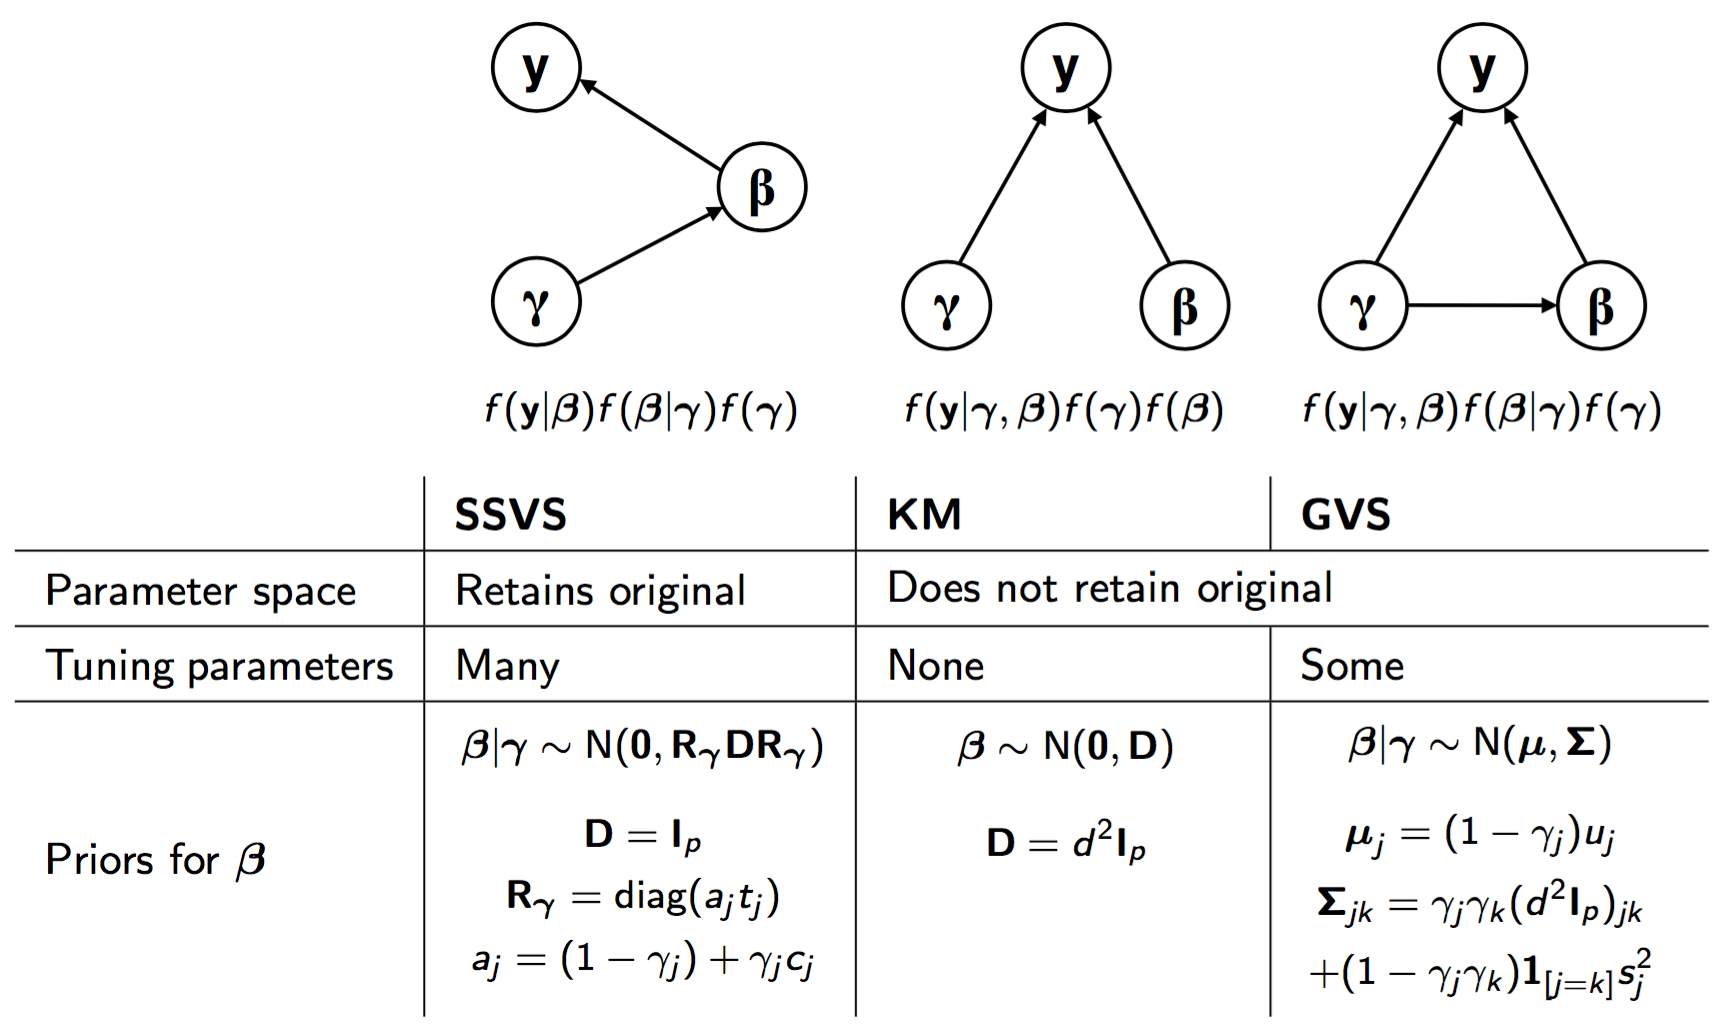
\includegraphics[scale=0.24]{figure/modcompare}
	\caption{A summarised comparison of the three Bayesian variable selection methods. Graphical models are also illustrated for each method.}
	\label{fig:modcompare}
\end{figure}

We now see an opportunity to use I-priors in the Bayesian variable selection methods, by simply replacing the prior covariance matrix $\mathbf D = d^2\mathbf I_p$, or in the case of SSVS $\mathbf D= \mathbf I_p$, by that of the I-prior covariance matrix $\psi\boldsymbol\Lambda \mathbf X ^\top \mathbf X \boldsymbol\Lambda$ (see the end of Section \ref{sec:scale}). \cite{George1993} have already suggested to use $\mathbf D \propto \mathbf (\mathbf X ^\top \mathbf X)^{-1}$ as a means of replicating the design correlation, and this turns out to be a generalisation of the g-prior for $\boldsymbol\beta$, though it seems to have the opposite effect. This is discussed in Section \ref{sec:gprior}. 

The question is which of the three methods shall we peruse I-priors? The unappealing feature of SSVS is the need to set the tuning parameters before running the model. \cite{George1993} do give four possible suggestions in their paper, but this is thought to be non-exhaustive. In other words, the user must really know the optimal settings for their problem at hand before running the variable selection model. On this note, GVS also has some tuning parameters to set, but not as many in our opinion. As the prior for $\boldsymbol\beta$ comprises of a true prior and pseudo prior. The obvious choice for the true prior is the I-prior (if we want to employ I-priors, that is). As for the pseudo prior, \cite{Ntzoufras2008} uses the estimates obtained from a full pilot MCMC run (see Section \ref{sec:dellaportas}) in his examples, and this seems reasonable. 

\stepcounter{todocounter}
\todo[caption={\thetodocounter. The use of I-priors in Bayesian variable selection needs more convincing theoretical justification.}]{More justification required}
Out of all these methods, KM stands out as being the simplest. I-priors fit straight into the story by replacing the prior on $\boldsymbol\beta$ in the model. We think this simplicity outweights the efficiency claimed to be brought about by introducing a pseudo prior in GVS. Further, the KM entails only specifying choices for the hyperparameters of the model as we would if we were estimate the linear model in a Bayesian manner. Since we are using the I-prior, there is no more hyperparameters to choose. This is a nice feature seeing it from a ``hands-free plug-and-play'' perspective.

The I-prior Bayesian variable selection model is given below:
\begin{align}\label{eq:ipriorbvs}
	\begin{gathered} 
		y_i = \alpha + \gamma_1\beta_1 x_{i1} + \dots + \gamma_p\beta_p x_{ip} + \epsilon_i \\
		\epsilon_i \sim \text{N}(0, \psi^{-1})  \\
		i=1,\dots,n\\
		\\
		\text{\underline{Priors}} \\
		\boldsymbol\beta \sim \text{N}(\mathbf 0, \psi\boldsymbol\Lambda \mathbf X ^\top \mathbf X \boldsymbol\Lambda), \text{ where } \boldsymbol\Lambda = \text{diag}[\lambda_1, \dots, \lambda_p]\\
		\gamma_j \sim \text{Bern}(p_j), \ j=1,\dots,p \\
		\alpha \sim \N(a,b^2) \\
		\psi, \lambda_1^{-2}, \dots,  \lambda_p^{-2} \sim \Gamma(c,d) \\
	\end{gathered}
\end{align}
By virtue of the I-prior being a maximum entropy prior, meaning that it is suitable to be used in the absence of prior information, we then complete the model specification above by also choosing uninformative hyperpriors (see Section \ref{sec:priorchoices}).

The scale parameters $\lambda_1, \dots, \lambda_p$ originally came from I-prior modelling in a function space framework, whereby these scale parameters help resolve the arbitrary scale of the space of functions over the set of covariates. As these scale parameters make their way into the covariance matrix of the $\boldsymbol\beta$ prior, we can interpret them as follows: if no scale parameters are introduced, or equivalently all scale parameters are equal to one, then the covariance matrix is proportional to $\mathbf X^\top \mathbf X$. As the covariates are likely to be measured on differing scales, such as age in years, height in metres, weight in kilograms, etc., the entries of $\mathbf X^\top \mathbf X$ will be large for measurements on a large scale range (e.g. body weight in grams), and small for measurements on a small scale range (e.g. body height in metres). This in turn affects the precision of the prior and consequently the estimation of the $\boldsymbol\beta$ parameter. For instance, a high precision (small variance) supports the predictor not being selected. What is ideal for us is that important variables should have $\beta_j$s estimated as non-zero and vice-versa, but simply putting $\mathbf X^\top \mathbf X$ as the covariance matrix does not contribute towards this goal. Therefore, scaling the prior covariance matrix of $\boldsymbol\beta$ is necessary, and the I-prior method of scaling is a natural choice here.

An alternative solution, as is practiced by the three methods in the previous section, is to standardise both the $\mathbf X$ and $\mathbf y$ variables. This is indeed a good idea, but is slightly unsatisfactory - scaling the variables so that each has variance one feels ad-hoc in the face of it. Having scale parameters estimated through the model seems more elegant and conforms more to the original I-prior methodology. Having said that, standardising the variables while using a single estimable scale parameter $\lambda$ is certainly an option, as all the variables would then have been scaled equally via standardisation. This has the advantage of taming extremely large entries of $\mathbf X^\top \mathbf X$ which may be problematic computationally when we require the inverse.\label{sec:bvsiprior}

\begin{remark}
	On another note, it might also possible to treat the scale parameters $\lambda_1, \dots, \lambda_p$ as fixed, having being estimated from the full model using the original I-prior framework described in Section \ref{sec:iprior}. This is an idea yet to be explored, and is not known whether this would yield good results. There is also a convergency and accuracy issue in obtaining reliable estimates of a large number of scale parameters through the EM procedure of maximising the likelihood of the I-prior model.
\end{remark}

We can estimate this model by Gibbs sampling. Unlike the KM model however, one of the Gibbs conditional posterior was not found to be in closed form, which was the posterior for the precision $\psi$. So to estimate this model, one has to incorporate a Metropolis-Hastings step for the estimation of $\psi$. The conditional posterior densities are given in Appendix \ref{apx:gibbs}. We can also feed this model into WinBUGS or JAGS which is then able to estimate this model for us.

\vspace{-2mm}
\subsection{Simulation study}
\vspace{-2mm}

\stepcounter{todocounter}
\todo[caption={\thetodocounter. Under what conditions exactly are I-priors advantageous to be used for Bayesian variable selection? Design further simulation studies to gain insight.}]{More simulations required}
\stepcounter{todocounter}
\todo[caption={\thetodocounter. How does the LASSO variable selection compare against I-priors?}]{Compare LASSO}
In this section, we compare the performance of the four methods of Bayesian variable selection: SSVS, KM, GVS, and I-prior by means of a simulation study. The experiment is to select from $p=100$ variables of a $n=150$ sample size artificial dataset which has pairwise correlations between the variables. This was inspired by the studies done by \cite{George1993} and \cite{Kuo1998} in their respective papers, albeit on a larger scale (in theirs, $p=30$).

The data was generated as follows:
\begin{itemize}
	\item Draw $\mathbf Z_1, \dots, \mathbf Z_{100} \sim \text{N}(\mathbf 0, \mathbf I_{150})$.
	\item Draw $\mathbf U \sim \text{N}(\mathbf 0,\mathbf I_{150})$.
	\item Let $\mathbf X_j = \mathbf Z_j + \mathbf U$. This induces pairwise correlations of about 0.5.\footnotemark
	\item Draw $\boldsymbol \epsilon \sim \text{N}(\mathbf 0, 2^2\mathbf I_{150})$.
	\item Generate response variables $\mathbf Y = \mathbf X \boldsymbol\beta_{\text{true}} + \boldsymbol\epsilon$.
\end{itemize}

\footnotetext{$\text{Cov}(X_j, X_k) = \text{Cov}(Z_j + U, Z_k + U) = \text{Var } U = 1$, and $\text{Var}(X_j) = \text{Var}(Z_j + U) = 2$. Thus, $\text{Corr}(X_j, X_k) = \text{Cov}(X_j, X_k) / (\text{Var}(X_j)\text{Var}(X_k))^{1/2} = 1/2$.}

Let $\boldsymbol\beta_{\text{true}} = (\boldsymbol\beta_{-k}, \boldsymbol\beta_{k})$, where $\boldsymbol\beta_{-k} = (\beta_1, \dots, \beta_k) = (0,\dots,0)$ and $\boldsymbol\beta_{k} = (\beta_{k+1}, \dots, \beta_{100}) = (1,\dots,1)$. In other words, only variables $X_{k+1}$ to $X_{100}$ are used. The experiment involves varying the value of $k$ between 10, 25, 50, 75 and 90 to create five scenarios, which we label as Scenarios A to E respectively. The two extremes, Scenarios A and E, are meant to simulate situations in which there are a lot of non-zero betas in the true model (Scenario A) and situations in which there are very few non-zero betas in the true model (Scenario E). The variable selection is conducted with many correlated variables.

10,000 MCMC were samples obtained for each scenario, and the metric of interest is the number false choices the models make, i.e. selecting variables which were not in the true model and failing to select variables which were in the true model. Each experiment was repeated 10 times and results averaged, as this ensures that a good result  was not simply due to chance of a good random seed in the data generation step. This experiment was conducted in R using JAGS, a variation of WinBUGS, and the results presented in the form of histograms in Figure \ref{fig:simres1}. Note that the same prior for $\boldsymbol{\beta}$ was used in the KM and GVS method, so we expect the results to be similar for these two methods.

\begin{figure}
	\centering
	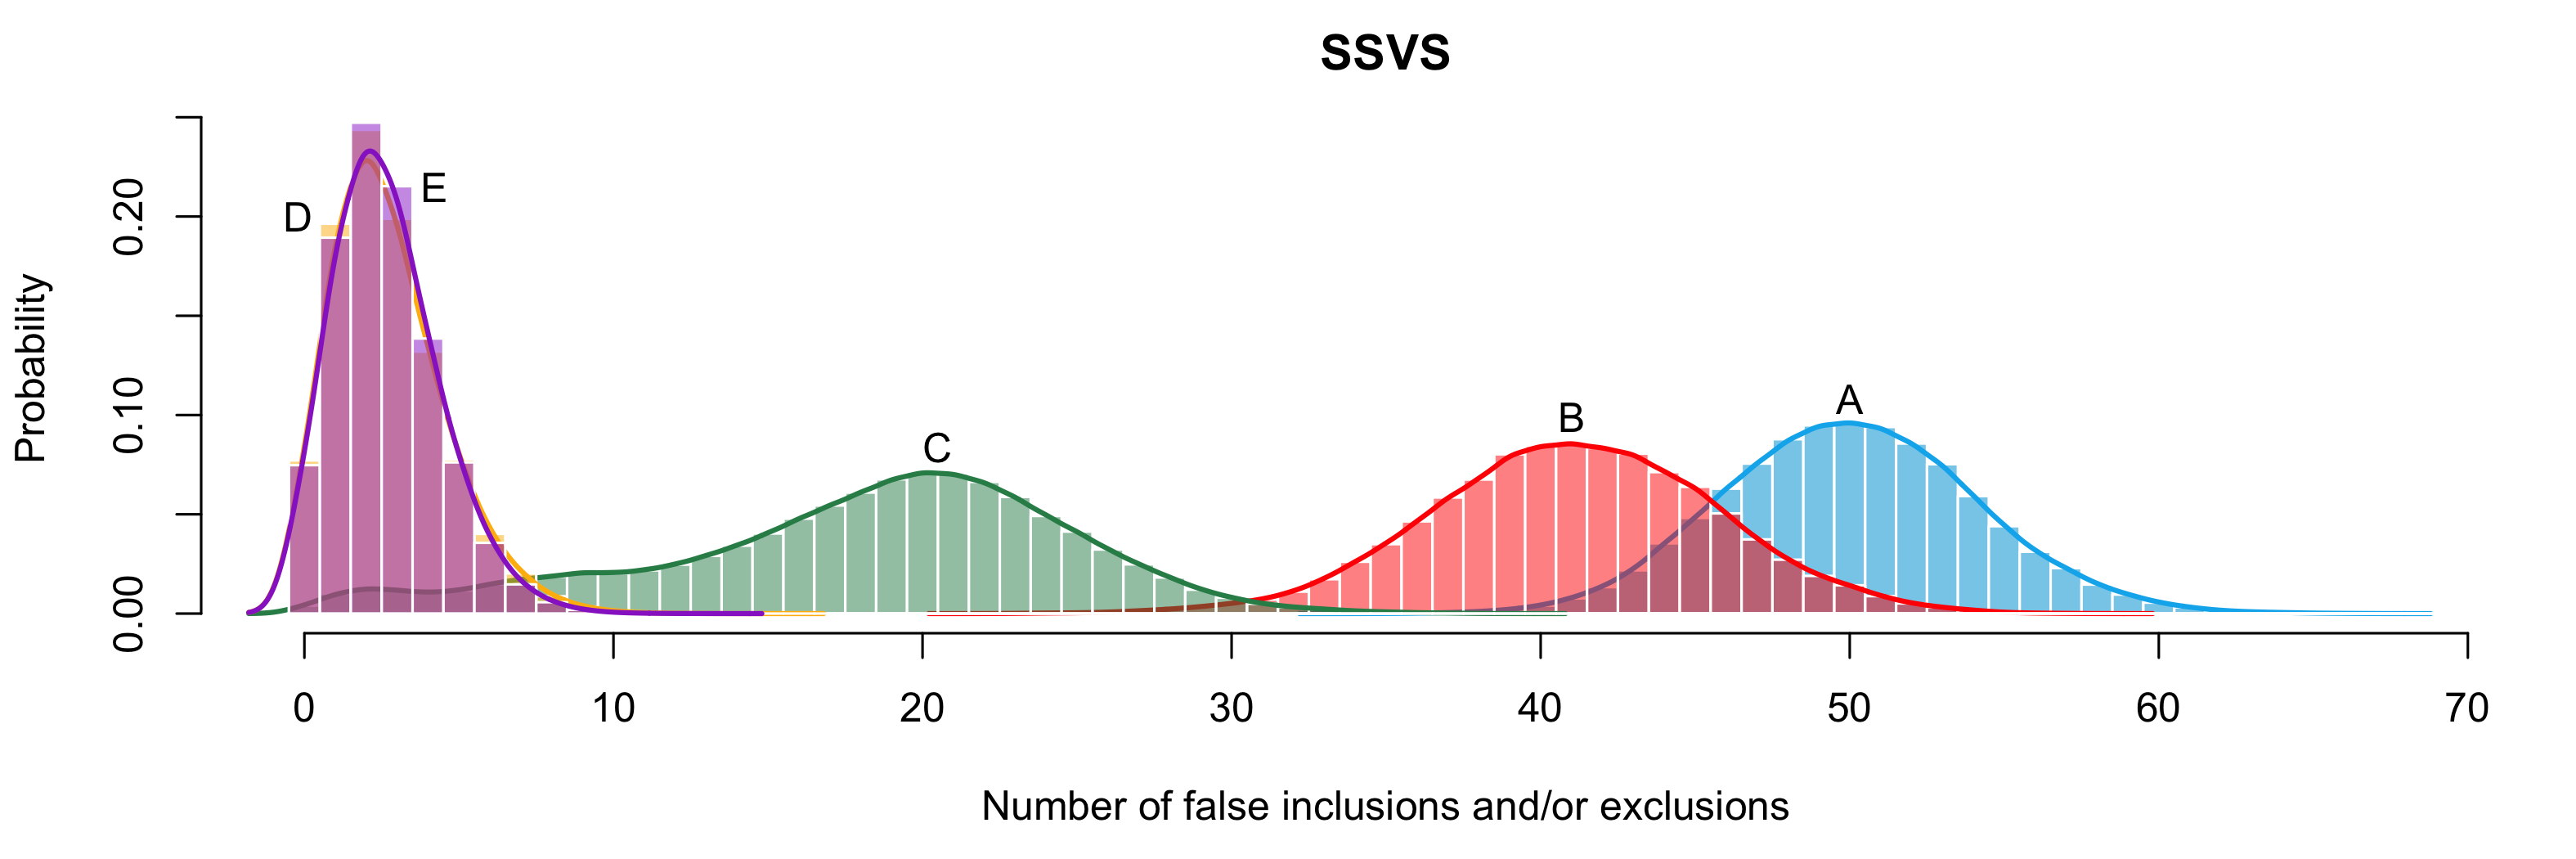
\includegraphics[width=6in, height=1.95in]{figure/sim1}
	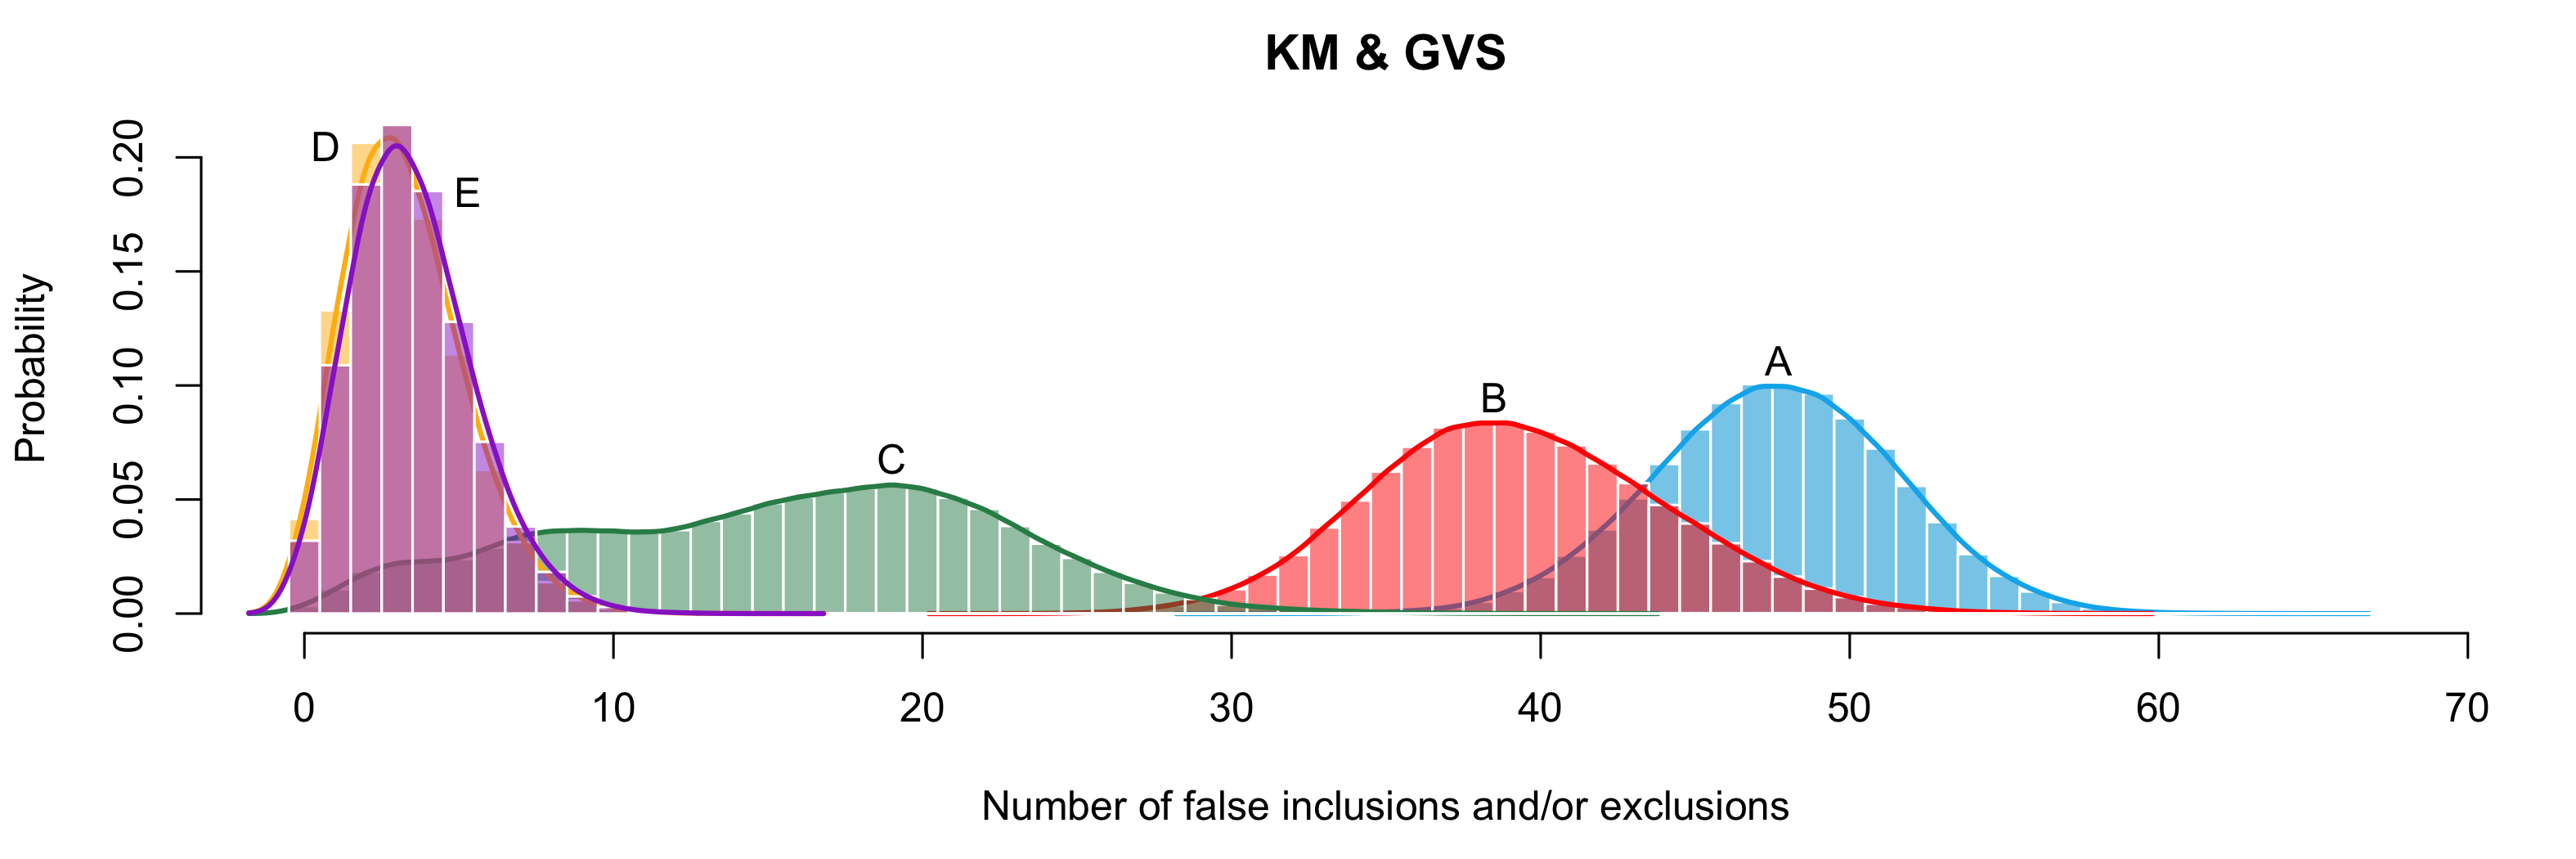
\includegraphics[width=6in, height=1.95in]{figure/sim2}
	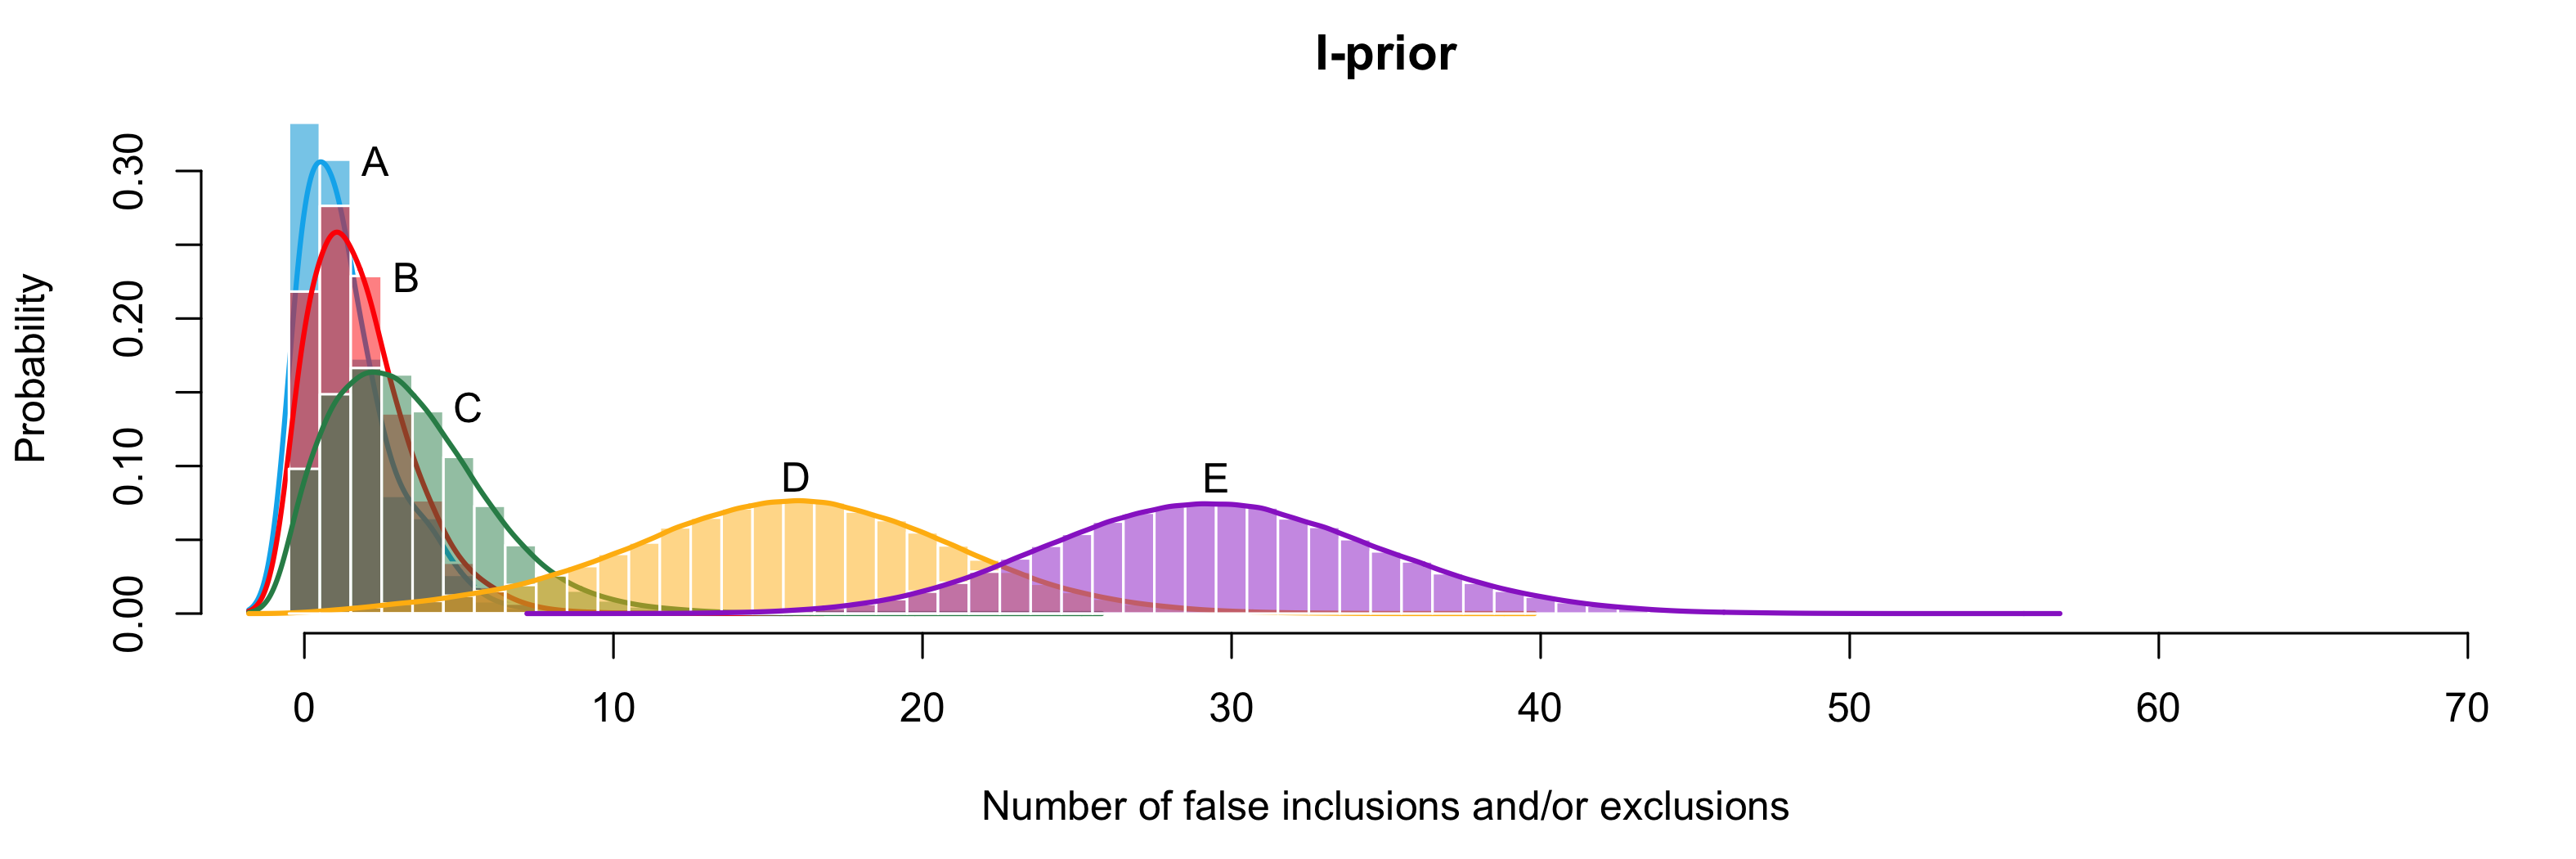
\includegraphics[width=6in, height=1.95in]{figure/sim4}
	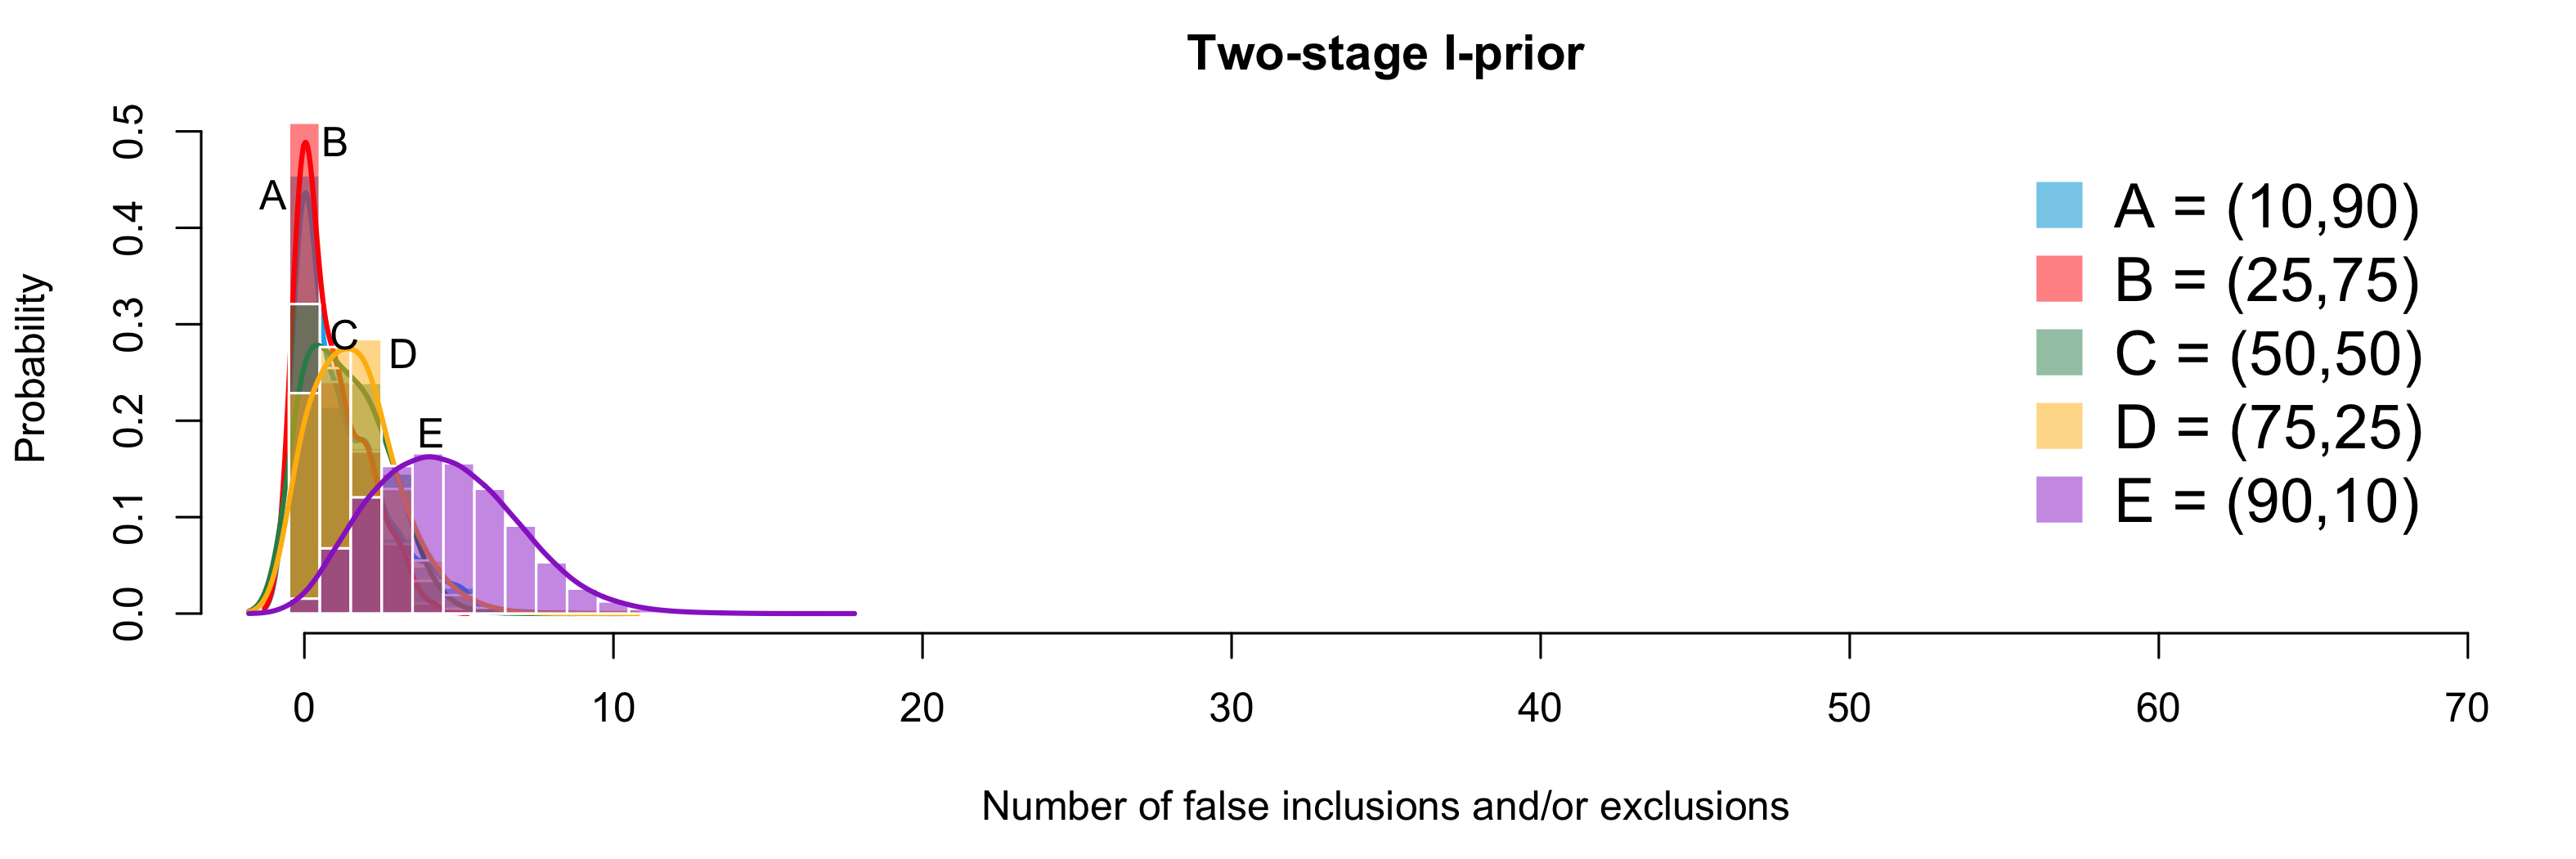
\includegraphics[width=6in, height=1.95in]{figure/sim5}
	\\ \vspace{-10pt}		
	\caption{Histograms of false choices for SSVS, KM (equivalent to GVS), I-prior and two-stage I-prior compared across the five scenarios A to E. Each scenario is labelled as ``$(k, 100-k)$'', where $k$ denotes the number of zeros in the true value of $\boldsymbol{\beta}$ used.}
	\label{fig:simres1}
\end{figure}

The ideal picture would be a histogram with a lot of mass towards the left side of the graph, indicating models which produced little false choices. The histograms indicate similar behaviour for the SSVS, KM and GVS methods. These methods perform poorly in the presence of many non-zero $\boldsymbol\beta$s, but perform slightly better in the presence of few non-zero $\boldsymbol\beta$s. For I-priors however, it is the opposite situation. The I-prior method seems to work quite well given many non-zero $\boldsymbol\beta$s, but performance worsens when there are actually few non-zero $\boldsymbol\beta$s in the true model. However, in the defence of I-priors, when it does well in Scenarios A, B and C, it does much better (fewer false choices) than when the other three methods do well (Scenarios D and E). I-prior is also less worse than when the other methods do terribly (maximum number of false choice for I-prior is 30, compared to $\approx50$ for any of the other three methods).

One possible explanation here is that when there are a lot of zero $\boldsymbol\beta$s in the true model, the Fisher information in the covariance matrix of the prior only serves to confuse with all this evidently unnecessary information. Hence, we can't expect I-priors to benefit in situations like these. Scenarios D and E bode well for the other three methods because the lack of a correlation structure in the covariance matrix of the priors causes these methods to select fewer variables, and thus make fewer false choices.

\subsection{Two-stage procedure}

Since I-priors do quite well in Scenarios A-C, but not in D and E, why don't we try to make Scenarios D and E a bit more like Scenarios A-C? This requires some sort of pre-selection of the variables in order to trim off the unwanted variables before running the variable selection model. Without appealing to other pre-selection methods, there is some information from the Bayesian variable selection models that we can make use of - the posterior inclusion probabilities for each variable. As this gives an overall indication as to how valuable a particular variable is, we look for ways to incorporate this into our decision-making process of pre-selecting the variables. The obvious solution is to run the model twice:
\begin{itemize}
	\item [\textbf{1st}] Run the model. Discard variables with posterior inclusion probabilities less than $\tau$, a treshold value.
	\item [\textbf{2nd}] Re-run the model on the set of reduced variables.
\end{itemize}

%\begin{sidewaysfigure}
%	\begin{center}
%		\includegraphics[scale=0.36]{figure/simres2}	
%		\caption{Histogram of results for the two-stage procedure using I-priors. An improvement is seen across all scenarios, as the histograms shift towards the left.}
%		\label{fig:simres2}
%	\end{center}
%\end{sidewaysfigure}

A natural choice for $\tau$ would be 0.5. Setting it at 0.5 would mean that we only keep variables which have a better than equal chance of being selected. The model such that all posterior inclusion probabilities are greater than or equal to 0.5 is known as the median probability model. While this value of 0.5 may seem slightly arbitrary to some, \cite{Barbieri2004} had done some work on median probability models, for which they had shown that under certain strict conditions, these models are also the most optimally predictive models that is able to be selected. The notion of two-stage procedures are not new, as many variable selection methods in the literature generally employ a pre-selection method before running their methods proper. For a two-stage procedure based on posterior inclusion probabilities, \cite{Fouskakis2008} and \cite{Ntzoufras2008} have employed this in their work.

The histogram at the bottom of Figure \ref{fig:simres1} shows that this two-stage procedure does indeed improve on the I-prior method. We see that a shift in the histogram towards the left-hand side of the graph for the second stage run of the model. Interestingly, not only does this improve the Scenarios D and E, we also seem improvements for Scenarios A-C. 

\begin{remark}
	Among the reasons for a pre-selection of the variables are to remove highly correlated variables, removing variables which have no theoretical benefit, or simply to reduce the large number of variables for large especially when $p > n$. There is probably no justification why a two-stage procedure would work better than just a one-stage procedure other than for convenience. At the end of the day, it is the responsibility of the user to interpret the results of the variable selection methods carefully and not make inference blindly on the results of the model.
\end{remark}

\subsection{Real world applications}

Here we look at three real-world applications on problems where there are some degree of multicollinearity in the datasets, and have been looked at before from a variable selection standpoint so that we are able to compare results to I-priors.

\subsubsection{Aerobic fitness data}

This dataset appeared in the \textit{SAS/STAT\textsuperscript{\textregistered} User's Guide} \cite{SAS2008} and was also analysed by \cite{Kuo1998}. It involves understanding the factors which affect aerobic fitness, which is measured by the ability to consume oxygen. A sample of $n=30$ male participants' had their physical fitness measured by means of simple exercise tests. The response variable \texttt{Oxygen} contains measurement of oxygen uptake rate in mL/kg body weight per minute. The six covariates were the participants' \texttt{Age}, \texttt{Weight}, time taken to run one mile (\texttt{RunTime}), resting heart rate (\texttt{RestPulse}), heart rate while running (\texttt{RunPulse}), and maximum heart rate during the exercise (\texttt{MaxPulse}). This dataset, although small in size, is interesting to analyze because of the correlations between the variables, mainly due to the measurements being taken during the same exercise test. The sample correlations of interest are shown in Figure \ref{fig:aerobic-cor} below:

\begin{figure}[H]
	\centering
	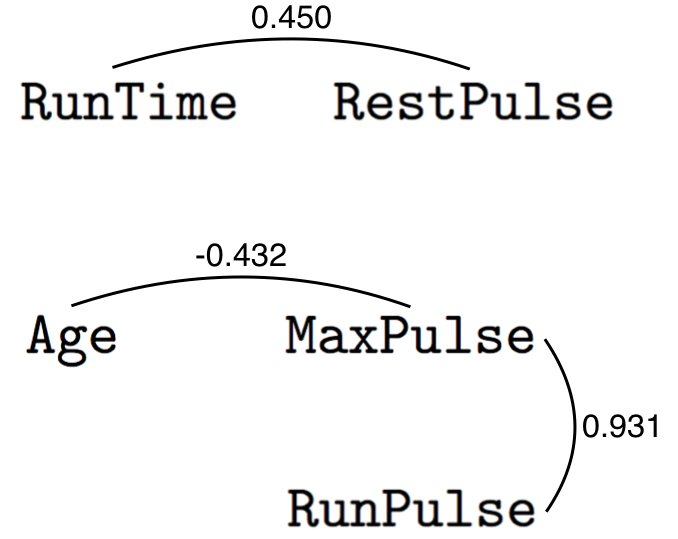
\includegraphics[height=1.3in]{figure/aerobic-cor}
	\caption{The sample correlations of interest in the aerobic fitness dataset. These show variables with correlations greater than 0.4 in magnitude. \label{fig:aerobic-cor}}
\end{figure}

The SAS analysis employed a forward selection and backwards elimination procedure and concluded that variables \texttt{Weight} and \texttt{RestPulse} were to be deleted. The KM procedure concurred with this finding. The I-prior method also did not choose the \texttt{Age} variable in addition to \texttt{Weight} and \texttt{RestPulse} in the maximum probability model. The variable \texttt{Age} only had a probability of 0.05 of being included in any posterior model, and also failed to appear in the top 92\% of likely models. This can be explained by the correlation between \texttt{Age} and \texttt{MaxPulse} - supposedly the information encoded in \texttt{Age} has already been taken care of by \texttt{MaxPulse}, so the I-prior deemed this as surplus. However, the models that had \texttt{Age} selected performed better in terms of AIC, Mallows $C_p$, and 5-fold cross validation root mean squared error (RMSE). Despite this, the strength of the coefficients for the variables are comparable to that of the I-prior method, which is settling if one wishes to do inference on this.

{\scriptsize
\begin{table}[H]
\centering
\begin{tabular}{l|rrrr}
					&\textbf{Full model}					
					&\textbf{I-prior}		
					&\textbf{Forward sel.}					
					&\textbf{Back elim.} \\
\hline
\texttt{Intercept}	&104.2 (0.00) 				&80.8 (0.00)		&103.3 (0.00) 				&98.6 (0.00) \\
\texttt{Age}			&-0.24 (0.03) 				&				&-0.25 (0.02) 				&-0.21 (0.05) \\
\texttt{Weight}		&{\color{gray!60}-0.08 (0.15)} 	&				&{\color{gray!60}-0.08 (0.15)} 	& \\
\texttt{RunTime}		&-2.59 (0.00) 				&-2.97 (0.00)	&-2.64 (0.00) 				&-2.75 (0.00) \\
\texttt{RestPulse}	&{\color{gray!60}-0.02 (0.72)} 	&				&			 					& \\
\texttt{RunPulse}		&-0.38 (0.00) 				&-0.38 (0.01)	&-0.39 (0.00) 				&-0.36 (0.01) \\ 
\texttt{MaxPulse}		&0.32 (0.03) 				&0.36 (0.02)	&0.32 (0.03) 					&0.28 (0.05) \\
\hline
$C_p$				&7.0 		&7.7		&5.1 		&5.3 \\
AIC					&56.8 		&58.5 	&54.9 		&55.6 \\
5f-CV RMSE		&2.59		&2.71 	&2.50		&2.54 \\
\end{tabular}
\caption{The OLS estimates for each variable are given in the table above, along with the standard errors in parantheses. The table also shows the value for Mallow's $C_p$, AIC and 5-fold cross validation RMSE given for each model.}
\end{table}
}
	
\subsubsection{Mortality and air pollution data}
\label{sec:airpollution}

The next real world application comes from a paper by \cite{McDonald1973}. In it, the effects of air pollution on mortality in a US metropolitan area ($n=60$ and $p=15$) were studied. The response variable is \texttt{Mortality}, a total age adjusted mortality rate, and the main pollution effects of interest were that of hydrocarbons (\texttt{HC}), oxides of nitrogen (\texttt{NOx}) and sulphur dioxide (\texttt{SO2}). Several other environmental and socioeconomic considerations were taken into account, otherwise the model may include unexplained variation which may have been caused by factors other than pollution. For example, a metropolitan area with a high proportion of the elderly should expect to have a higher mortality rate than one with a lower proportion. All of the variables can be considered as continuous and real. A full description of the data can be found in Appendix \ref{apx:airpollution}. 

This dataset also contains several highly correlated variables. When the full model is fitted, none of the pollutant effects were found to be significant. Clearly a variable selection method was required. \citeauthor{McDonald1973} used ridge regression analysis to determine which variables to select. We also have results from a backwards elimination procedure (using AIC as the selection criterion) for comparison. The results are summarised in Table \ref{tab:poll}.

{\footnotesize
\begin{table}[H]
\centering
\begin{tabular}{m{0.4cm}|m{0.3cm}|m{2.5cm}|m{2.9cm}|m{2.6cm}|m{2.0cm}}
					\multicolumn{2}{l|}{}
					&\textbf{Full model}					
					&\textbf{I-prior}		
					&\textbf{Ridge}
					&\textbf{Back elim.}	\\
\hline
\multicolumn{2}{l|}{\parbox{2.0cm}{\centering\scriptsize{Environmental \& demographic variables selected}}}	
&{\small All, but only} \newline \texttt{Rain}, \texttt{JanTemp}, \newline \texttt{NonW} {\small significant}
&\texttt{Rain}, \texttt{JanTemp}, \newline {\color{gray}\texttt{JulTemp}}, {\color{gray}\texttt{Over65}}, \newline {\color{gray}\texttt{Popn}}, {\color{gray}\texttt{Hous}}, \texttt{NonW}, \newline {\color{gray}\texttt{Poor}}, {\color{gray}\texttt{Humid}}
&\texttt{Rain}, \texttt{JanTemp}, \newline \texttt{Educ}, {\color{gray}\texttt{Dens}}, \newline \texttt{NonW} 
&\texttt{JanTemp}, \texttt{Educ}, \texttt{NonW} \\
\hline
\parbox[t]{1cm}{\multirow{3}{*}{\rotatebox[origin=c]{90}{\parbox{1cm}{\centering\tiny{Pollution effect}}}}} 	
& \texttt{HC}		&{\color{red}\xmark} 		&{\color{red}\xmark}		&{\color{red}\xmark}		&{\color{green}\cmark} \small{$\beta = -0.98$} \\
& \texttt{NOx}	&{\color{red}\xmark}		&{\color{red}\xmark}		&{\color{red}\xmark}		&{\color{green}\cmark} \small{$\beta = 1.99$} \\
& \texttt{SO2} 	&{\color{red}\xmark}		&{\color{green}\cmark} \small{$\beta = 0.33$}	&{\color{green}\cmark} \small{$\beta = 0.24$}	&{\color{red}\xmark}	\\
\hline
\multicolumn{2}{l|}{$C_p$}	
&16.0	&13.4	&5.6		&8.7 \\
\multicolumn{2}{l|}{AIC}	
&439.8	&439.2	&431.3	&435.0 \\
\multicolumn{2}{l|}{BIC}	
&49.5	&36.5	&20.3	&21.2 \\
\multicolumn{2}{l|}{5f-CV RMSE}
&50.6		&41.7		&39.3		&38.6 \\
\end{tabular}
\caption{The results of the various variable selection methods compared. For each method, the variable selection procedure was conducted on the set of all variables, and then an OLS was fit on the resulting selected variables. The environmental and demographic variables selected are shown in the table for each model, but those in gray are the ones found to be not significant (at the 10\% level). \label{tab:poll}}
\end{table}
}

\vspace{-4mm}
It is noted that the I-prior method selected some variables which turned out to be insignificant, with only three significant variables selected in total. However, of importance is learning which of the three pollution factors has an effect on mortality rate. It is nice to see that the I-prior agrees with the ridge analysis done by \citeauthor{McDonald1973} on this, with only sulphur dioxide having a significant effect. The strength of this effect is also comparable (I-prior 0.33 c.f. ridge 0.24). The method of backwards elimination was found not only inconsistent with I-prior and ridge analysis, but also erroneous in that it seems to imply an increase in levels of hydrocarbons would bring about a reduction in mortality rate. Once again, we see that the I-prior is outperformed in terms of Mallow's $C_p$, AIC, BIC and 5-fold CV RMSE, but it is noted that the 5-fold CV RMSE is not too far off from its competitors. 

\vspace{-2mm}
\subsubsection{Ozone data}
\label{sec:ozone}
\vspace{-1mm}

In this section, we replicate the Bayesian variable selection analysis of the Ozone dataset done by \cite{Casella2006} which appeared initially in \cite{Breiman1985}, and also show how Bayesian variable selection can help select important interaction terms. The data consists of daily ozone readings and various meteorological quantities, and the aim was to see which of these quantities contributed to the ozone concentration. The variables are explained in Appendix \ref{apx:ozone}. 

The data contains 366 points, one for each day of the leap year 1976. For our analysis, we ignore the 163 missing data in the set, and use the remaining 203 datapoint for our analysis. Out of these 203, we randomly set aside 25 to use for validation. So the $n$ used for the Bayesian variable selection methods was $n=178$. \citeauthor{Casella2006} removed the variables \texttt{TempElMon} and \texttt{ibtLAX} before running their selection model, citing multicollinearity. We won't do this, as we would like to see how well I-priors do in the presence of multicollinearity. On another note, the variables \texttt{Month}, \texttt{DayMonth} and \texttt{DayWeek} were presumably intended to be categorical as in modelling seasonality in a time series data, but these were treated as continuous, as did \citeauthor{Casella2006}. This is just as well, as our I-prior model is not able to handle categorical variables which have more than two levels. The results are compared below:

\begin{table}[h]
\centering\small
\begin{tabular}{l|lrrr}
Method      & Model                           & Post. prob.     & $R^2$		& RMSE  \\
\hline
I-prior     & \texttt{Month HumLAX TempElMon}          & 0.544           & 0.72     & 3.86 \\
CM (MPM)  & \texttt{HumLAX TempSand ibhLAX}          & \textless 0.001 & 0.69     & 4.47 \\
CM (MSE)  & \texttt{Month HumLAX TempSand ibhLAX}    & \textless 0.001 & 0.70     & 4.04 \\
BF & \texttt{TempSand ibhLAX PresGrad VisLAX} & \textless 0.001 & 0.66     & 4.27
\end{tabular}
\caption{Table showing the comparison between the I-prior, Casella and Moreno (CM) analysis, and the ACE method by Breiman and Friedman (BF). MPM stands for maximum probability model, and MSE is the lowest RMSE model.}
\label{tab:ozoneres}
\end{table}

The maximum probability I-prior model was found to be much better in terms of RMSE compared to the maximum probability model of \citeauthor{Casella2006}. The variables selected using I-prior corresponded to the significant variables when the full OLS model was fitted. Our I-prior selected model also had a lower RMSE than \citeauthor{Casella2006}'s lowest RMSE model. The ACE method by \citeauthor{Breiman1985} was found to be the worst model for prediction. It is noted that neither \citeauthor{Casella2006}'s nor \citeauthor{Breiman1985}'s model were found in the posterior model space using the I-prior method. Out of interest, if we had removed the two variables \texttt{TempElMon} and \texttt{ibtLAX} at the beginning, then we arrive at the same results as \citeauthor{Casella2006}.

We now use the I-prior method to select between the squared terms and all level two interactions in an effort to improve model prediction. For 12 such variables, the number of variables to select becomes $12 + 12 + 12(12 - 1)/2 = 90$. By doing so, we were able to improve the model to give a slightly better predictive ability. The results are shown below in Table \ref{tab:resozone2}. The maximum probability model for I-prior method selected fewer variables as compared to \citeauthor{Casella2006}'s maximum probability model, yet was superior in terms of RMSE. For comparison, the backwards elimination resulted in a very complicated model which did not seem to improve on RMSE.

\begin{table}[h]
\centering\small
\begin{tabular}{p{1.1cm}|m{7.5cm}rrr}
Method      & Model                           & Post. prob.     & $R^2$		& RMSE  \\
\hline
I-prior        & \texttt{Month Month\textasciicircum2 WindLAX HumLAX  TempElMon TempElMon\textasciicircum2 ibtLAX PresGrad\textasciicircum2 ibtLAX:HumLAX}	& 0.103	& 0.83	&3.74 \\
\hline
CM     &  \texttt{DayMonth Month\textasciicircum2 TempSand\textasciicircum2 PresGrad\textasciicircum2 Month:WindLAX DayMonth:HumLAX DayWeek:TempSand PresVand:HumLAX HumLAX:ibhLAX HumLAX:VisLAX}                                                                                                                                                                                                                                                                                                                                                                 & \textless 0.001 & 0.76  & 3.88    \\
\hline
Back. elim. & \texttt{Month Month\textasciicircum2 DayWeek PresVand HumLAX TempSand TempSand\textasciicircum2 TempElMon ibhLAX VisLAX  PresVand\textasciicircum2 WindLAX\textasciicircum2  PresGrad\textasciicircum2 DayMonth:Month WindLAX:Month HumLAX:Month ibhLAX:Month ibtLAX:Month HumLAX:DayMonth TempSand:DayMonth TempElMon:DayMonth VisLAX:DayMonth WindLAX:PresVand HumLAX:PresVand TempSand:PresVand TempSand:WindLAX ibtLAX:WindLAX TempSand:HumLAX TempElMon:HumLAX VisLAX:HumLAX PresGrad:TempSand VisLAX:TempSand PresGrad:TempElMon VisLAX:TempElMon ibtLAX:PresGrad VisLAX:PresGrad} & \textless 0.001 & 0.87 &4.29   
\end{tabular}
\caption{Results of variable selection for to look for squared and interaction terms in the ozone dataset.}
\label{tab:resozone2}
\end{table}

\begin{remark}
	As the model fit involved randomly leaving out 25 data points which were later used for  validation, the results between our analysis and \citeauthor{Casella2006}'s are bound to differ, as we did not use the same 25 data points for training and testing.
\end{remark}



\begin{remark}
	For this particular dataset, running the model without squared terms and linear predictors was straightforward. However, we ran into a numerical issue in the second part, whereby some entries of $\mathbf X^\top \mathbf X$ were found to be so large compared to others, that its inverse could not be computed. Thus, we standardised the $\mathbf X$ and $\mathbf y$ variables and used a single scale parameter $\lambda$. See the second last paragraph of Section \ref{sec:bvsiprior} on page \pageref{sec:bvsiprior}.
\end{remark}

\begin{remark}
	The method that we employed was a naive I-prior variable selection method, whereby each of the 90 terms was considered independently. If one wishes a model such that its level one term is included when an interaction is present, then the variable selection needs to be adjusted accordingly. \cite{Kuo1998} gives an example of this:
\[
y_i = \alpha + \max(\gamma_1, \gamma_3)\beta_1x_{i1} + \max(\gamma_2, 
\]
\end{remark}
